\chapter{The Power of Geometry – Shapes, Spaces, and Measurement}

\section{Introduction: Why Geometry Matters}
Geometry is all around us. Every building, park, or road we see has some geometric form. When you arrange furniture in a room, measure the length of a wall, or even look at patterns in nature, you're interacting with geometric concepts.

Geometry helps us understand the properties of shapes and spaces, and how to measure and compare them. It’s one of the oldest branches of math, yet it remains one of the most practical.

In this chapter, we’ll explore the basics of geometry, focusing on shapes, angles, areas, and volumes, and how to apply these concepts in real-life situations.

\section{Basic Geometric Shapes and Their Properties}
Let’s start by getting familiar with the most common geometric ideas. Points are like the dot on a number line it has not length, widght or hight. Next we can think of a line of a set of continuous points. This line continues on in both directions to infinity. In Euclidean geometry, an angle is the figure formed by two rays, called the sides of the angle, sharing a common endpoint, called the vertex of the angle. Now lets consider 2D shapes (two-dimensional, flat shapes) and 3D shapes (three-dimensional, solid shapes).

\subsection{\textbf{Notation:}}
We use certain symbols and terms to describe geometric shapes and concepts. Here are some common ones:
\begin{table}[h!]
    \centering
    \begin{tabular}{|c|l|}
        \hline
        \textbf{Symbol} & \textbf{Meaning} \\ \hline
        $\alpha, \beta, \gamma$ & Angles \\ \hline
        $A, B, C$ & Vertices of a triangle \\ \hline
        $a, b, c$ & Sides of a triangle and the side of a square \\ \hline
        $r$ & Radius of a circle \\ \hline
        $h$ & Height of a triangle or the height of a cylinder \\ \hline
        $l$ & Length of a rectangle or the length of a rectangular prism \\ \hline
        $w$ & Width of a rectangle or the width of a rectangular prism \\ \hline
        $s$ & Side of a cube \\ \hline
        $d$ & Diameter of a circle \\ \hline
        $V$ & Volume of a 3D shape \\ \hline
        $P$ & Perimeter of a 2D shape \\ \hline
        $A$ & Area of a 2D shape \\ \hline
        $\pi$ & The constant pi, approximately 3.14159 \\ \hline
    \end{tabular}
    \caption{Notation used in Geometry}
    \label{tab:notation}
\end{table}

\subsection{Point}
A point represents a location in space. It has no length, width, or height.
We can represent a point visually as a dot on a coordinate plane:
\[
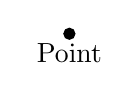
\begin{tikzpicture}
    \filldraw (0,0) circle (2pt);
    \node[below] at (0,0) {Point};
\end{tikzpicture}
\]

\subsection{Lines}
A line is a set of continuous points that extends infinitely in both directions. It has no thickness.
\[
\begin{tikzpicture}
    \draw (-2,0) -- (2,0);
    \node[below] at (0,0) {Line};
\end{tikzpicture}
\]

\subsection{Angle}
An angle is formed when two lines meet at a point. The size of an angle is measured in degrees. The degrees are notated with a small circle in the upper right corner of the number. Minutes and seconds are noted as follows: one degree is divided into 60 minutes (notated with a single quote, e.g., \(45^\circ 30'\)), and one minute is divided into 60 seconds (notated with a double quote, e.g., \(45^\circ 30' 15''\)).

\[
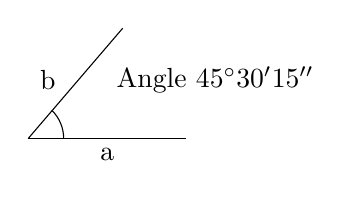
\begin{tikzpicture}
    % Draw the base line
    \draw (0,0) -- (2,0);
    \node[below] at (1,0) {a};
    % Draw the second line
    \draw (0,0) -- (1.2,1.4);
    \node[above] at (0.25,0.5) {b};
    % Add the angle label
    \node[right] at (1,0.75) {Angle \(45^\circ 30' 15''\)};
    % Draw the arc representing the angle
    \draw (0.45,0) arc[start angle=0, end angle=45.5042, radius=0.5];
\end{tikzpicture}
\]

\subsection{*Right Angle}
A right angle measures exactly 90 degrees. It looks like the corner of a square.
\textbf{Note:} The symbol for a right angle is a small square in the corner of the angle.
\[
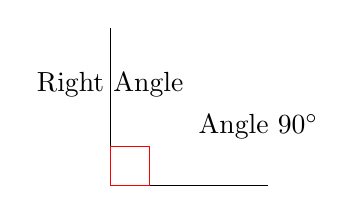
\begin{tikzpicture}
    % Draw the base line
    \draw (0,0) -- (2,0);
    \draw (0,0) -- (0,2);
    % Add the angle label
    \node[right] at (1,0.75) {Angle \(90^\circ\)};
    \node[above] at (0,1) {Right Angle};
    % Draw the square symbol for a right angle
    \draw[red] (0,0) rectangle (0.5,0.5);
\end{tikzpicture}
\]

\subsection{2D Shapes}
\subsubsection{Square}
\begin{itemize}
    \item All four sides are equal in length.
    \item Each angle is 90 degrees (a right angle).
    \item A is the length and hight of the square.
\end{itemize}

\[
\begin{tikzpicture}
    % Draw a square
    \draw (0,0) rectangle (2,2);

    % Draw right angle symbols inside the square
    \node (A) at (-.5,1) {A};
    \draw[red] (0,0) rectangle (0.5,0.5);
    \node (A) at (2.5,1) {A};
    \draw[red] (1.5,0) rectangle (2,0.5);
    \node (B) at (1,-.5) {A};
    \draw[red] (0,1.5) rectangle (0.5,2);
    \node (C) at (1,2.5) {A};
    \draw[red] (1.5,1.5) rectangle (2,2);

    % Add a label below the square
    \node[left] at (1.7,1) {Square};
\end{tikzpicture}
\]

\subsubsection{Rectangle}
\begin{itemize}
    \item Opposite sides are equal in length.
    \item Each angle is 90 degrees.
    \item A hight and B width of the rectangle.
\end{itemize}

\[
\begin{tikzpicture}
    \draw (0,0) -- (4,0) -- (4,2) -- (0,2) -- cycle;
    \node[below] at (2,1.25) {Rectangle};
    % Draw right angle symbols inside the square
    \node (A) at (-.5,1) {A};
    \draw[red] (0,0) rectangle (0.5,0.5);
    \node (A) at (4.5,1) {A};
    \draw[red] (3.5,0) rectangle (4,0.5);
    \node (B) at (2,-.5) {B};
    \draw[red] (0,1.5) rectangle (0.5,2);
    \node (C) at (2,2.5) {B};   
    \draw[red] (3.5,1.5) rectangle (4,2);
\end{tikzpicture}
\]
\subsubsection{Triangle}
\begin{itemize}
    \item A shape with three sides.
    \item The sum of the angles inside any triangle is always 180 degrees.
\end{itemize}
\[
\begin{tikzpicture}
    \draw (0,0) -- (2,4) -- (4,0) -- cycle;
    \node[below] at (2,0) {Triangle};
    \node[below left] at (0,0) {$A$};
    \node[above] at (2,4) {$B$};
    \node[below right] at (4,0) {$C$};
    \node[below left] at (1,2) {$\alpha$};
    \node[below right] at (3,2) {$\beta$};
    \node[above] at (2,1) {$\gamma$};
\end{tikzpicture}
\]

\[ 
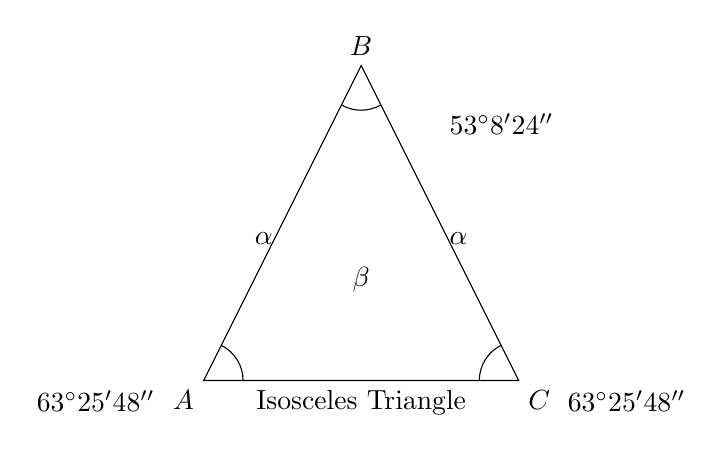
\begin{tikzpicture}
    \draw (0,0) -- (2,4) -- (4,0) -- cycle;
    \node[below] at (2,0) {Isosceles Triangle};
    \node[below left] at (0,0) {$A$};
    \node[above] at (2,4) {$B$};
    \node[below right] at (4,0) {$C$};
    \node[below left] at (1,2) {$\alpha$};
    \node[below right] at (3,2) {$\alpha$};
    \node[above] at (2,1) {$\beta$};
    \draw (.5,0) arc[start angle=0, end angle=63.43, radius=0.5];
    \draw (3.5,0) arc[start angle=180, end angle=116.57, radius=0.5];
    \draw (1.75,3.5) arc[start angle=240, end angle=300, radius=0.5];
    \node[above right] at (3,3) {\(53^\circ 8' 24''\)};
    \node[below left] at (-0.5,0) {\(63^\circ 25' 48''\)};
    \node[below right] at (4.5,0) {\(63^\circ 25' 48''\)};
\end{tikzpicture}
\]

\subsubsection{Equilateral Triangle}
\begin{itemize}
    \item A triangle with all sides of equal length.
    \item All angles are equal.
    \item Each angle measures 60 degrees.
    \item The sum of the angles inside any triangle is always 180 degrees.
    \item The sum of the angles inside an equilateral triangle is always 180 degrees.
\end{itemize}

\[
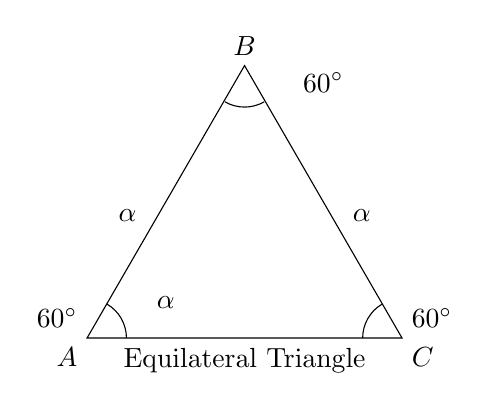
\begin{tikzpicture}
    \draw (0,0) -- (2,3.46) -- (4,0) -- cycle;
    \node[below] at (2,0) {Equilateral Triangle};
    \node[below left] at (0,0) {$A$};
    \node[above] at (2,3.46) {$B$};
    \node[below right] at (4,0) {$C$};
    \node[below left] at (.75,1.75) {$\alpha$};
    \node[below right] at (3.25,1.75) {$\alpha$};
    \node[above] at (,0.25) {$\alpha$};
    \node[below left] at (0,0.5) {$60^\circ$};
    \node[below right] at (4,0.5) {$60^\circ$};
    \node[above] at (3,3) {$60^\circ$};
    \draw (0.5,0) arc[start angle=0, end angle=60, radius=0.5];
    \draw (3.5,0) arc[start angle=180, end angle=120, radius=0.5];
    \draw (1.75,3) arc[start angle=240, end angle=300, radius=0.5];
\end{tikzpicture}
\]

\subsubsection{Scalene Triangle}
\begin{itemize}
    \item A triangle with all sides of different lengths.
    \item All angles are different.
\end{itemize}

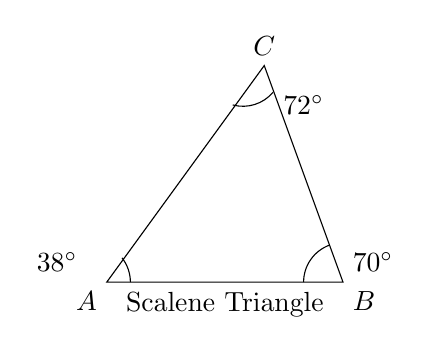
\begin{tikzpicture}
    \draw (0,0) -- (3,0) -- (2,2.75) -- cycle;
    \node[below] at (1.5,0) {Scalene Triangle};
    \node[below left] at (0,0) {$A$};
    \node[below right] at (3,0) {$B$};
    \node[above] at (2,2.75) {$C$};
    \node[below left] at (-0.25,0.5) {$38^\circ$};
    \node[below right] at (3,0.5) {$70^\circ$};
    \node[above] at (2.5,2) {$72^\circ$};
    \draw (0.3,0) arc[start angle=0, end angle=38, radius=0.5];
    \draw (2.5,0) arc[start angle=180, end angle=110, radius=0.5];
    \draw (1.6,2.25) arc[start angle=255, end angle=320, radius=0.5];
\end{tikzpicture}

\subsubsection{Circle}
\begin{itemize}
    \item A round shape where every point on the boundary is the same distance from the center.
    \item The distance from the center to the edge is called the radius.
    \item The total distance around the circle is called the circumference.
\end{itemize}

\subsection{3D Shapes}
\subsubsection{Cube}
\begin{itemize}
    \item All edges are equal, and it has 6 square faces.
\end{itemize}

\subsubsection{Rectangular Prism}
\begin{itemize}
    \item Like a cube, but with rectangular faces instead of square ones.
\end{itemize}

\subsubsection{Sphere}
\begin{itemize}
    \item A round 3D shape, like a ball. Every point on the surface is the same distance from the center.
\end{itemize}

\subsubsection{Cylinder}
\begin{itemize}
    \item A shape with two circular bases and straight sides.
\end{itemize}

\section{Understanding Perimeter and Area}
Perimeter is the distance around the outside of a shape. To find the perimeter, you simply add up the lengths of all the sides of a shape.

\subsection{Example}
To find the perimeter of a rectangle with a length of 5 units and a width of 3 units, add the lengths of all sides:
\[
\text{Perimeter} = 5 + 3 + 5 + 3 = 16 \text{ units}
\]

Area is the amount of space inside a 2D shape. Each shape has its own formula for calculating area.

\subsection{Formulas for Common Shapes}
\subsubsection{Square}
\[
\text{Area} = \text{side} \times \text{side}
\]
For example, if each side of a square is 4 units:
\[
\text{Area} = 4 \times 4 = 16 \text{ square units}
\]

\subsubsection{Rectangle}
\[
\text{Area} = \text{length} \times \text{width}
\]
If a rectangle has a length of 5 units and a width of 3 units:
\[
\text{Area} = 5 \times 3 = 15 \text{ square units}
\]

\subsubsection{Triangle}
\[
\text{Area} = \frac{1}{2} \times \text{base} \times \text{height}
\]
If a triangle has a base of 6 units and a height of 4 units:
\[
\text{Area} = \frac{1}{2} \times 6 \times 4 = 12 \text{ square units}
\]

\subsubsection{Circle}
\[
\text{Area} = \pi \times \text{radius}^2
\]
If a circle has a radius of 3 units:
\[
\text{Area} = 3.14 \times 3^2 = 28.26 \text{ square units} \quad (\text{where } \pi \approx 3.14)
\]

\section{Exploring Angles}
An angle is formed when two lines meet at a point. The size of an angle is measured in degrees.

\subsection{Types of Angles}
\begin{itemize}
    \item \textbf{Right angle:} Measures exactly 90 degrees (like the corners of a square).
    \item \textbf{Acute angle:} Measures less than 90 degrees.
    \item \textbf{Obtuse angle:} Measures more than 90 degrees but less than 180 degrees.
    \item \textbf{Straight angle:} Measures exactly 180 degrees.
\end{itemize}

You can measure angles using a protractor, which helps you see exactly how many degrees the angle has.

\section{Volume: Measuring 3D Shapes}
Just as we can measure the area of 2D shapes, we can measure the volume of 3D shapes. Volume tells us how much space is inside a 3D object, like how much water a box can hold.

\subsection{Formulas for Common 3D Shapes}
\subsubsection{Cube}
\[
\text{Volume} = \text{side} \times \text{side} \times \text{side}
\]
If each side of the cube is 3 units:
\[
\text{Volume} = 3 \times 3 \times 3 = 27 \text{ cubic units}
\]

\subsubsection{Rectangular Prism}
\[
\text{Volume} = \text{length} \times \text{width} \times \text{height}
\]
If a rectangular prism has dimensions of 4 units (length), 3 units (width), and 5 units (height):
\[
\text{Volume} = 4 \times 3 \times 5 = 60 \text{ cubic units}
\]

\subsubsection{Sphere}
\[
\text{Volume} = \frac{4}{3} \times \pi \times \text{radius}^3
\]
If the radius of the sphere is 2 units:
\[
\text{Volume} \approx \frac{4}{3} \times 3.14 \times 2^3 = 33.51 \text{ cubic units}
\]

\subsubsection{Cylinder}
\[
\text{Volume} = \pi \times \text{radius}^2 \times \text{height}
\]
If a cylinder has a radius of 3 units and a height of 5 units:
\[
\text{Volume} \approx 3.14 \times 3^2 \times 5 = 141.3 \text{ cubic units}
\]

\section{Real-Life Geometry: Applying What We’ve Learned}
Geometry has countless real-world applications. Here are a few examples:

\begin{itemize}
    \item \textbf{Architecture:} When designing a building, architects use geometric shapes to create floor plans, walls, and ceilings. They calculate areas to ensure the building materials fit properly.
    \item \textbf{Gardening:} If you want to fence a rectangular garden, you need to know the perimeter. If you’re planting flowers and want to cover the entire space, you’ll need to calculate the area.
    \item \textbf{Sports:} In sports like basketball, the area of the court determines the playing space, while the volume of the ball affects how it moves through the air.
    \item \textbf{Design:} When creating packaging for a product, designers must consider the volume of the box or container to ensure it holds the right amount of material.
\end{itemize}

\section{Practice Makes Perfect: Let’s Try Some Exercises!}
\subsection{Perimeter and Area}
\begin{itemize}
    \item Find the perimeter of a rectangle with a length of 7 units and a width of 4 units.
    \item Find the area of a triangle with a base of 8 units and a height of 5 units.
    \item Calculate the area of a circle with a radius of 6 units.
\end{itemize}

\subsection{Volume}
\begin{itemize}
    \item Find the volume of a cube with sides of 4 units.
    \item Calculate the volume of a rectangular prism with dimensions 3 units (length), 5 units (width), and 2 units (height).
    \item Find the volume of a cylinder with a radius of 3 units and a height of 7 units.
\end{itemize}

\subsection{Angles}
\begin{itemize}
    \item What type of angle measures 120 degrees?
    \item Measure the angle formed by the hands of a clock at 3:00.
\end{itemize}

\section{Chapter Summary}
\begin{itemize}
    \item Geometry helps us understand the shapes and spaces around us.
    \item We learned about basic 2D and 3D shapes and how to calculate their perimeters, areas, and volumes.
    \item We explored angles and how to measure them.
    \item Geometry is everywhere in our daily lives, from architecture to sports and design.
\end{itemize}

\subsection{Challenge Question}
You have a garden in the shape of a rectangle. The garden is 10 meters long and 6 meters wide. You want to fence the garden and plant flowers in the entire space. How much fencing will you need (perimeter), and how many square meters of flowers will you plant (area)?


